
\documentclass[a4paper]{article}

\usepackage[utf8]{inputenc}	% Flere sprog tegnsæt (fx æøå)
\usepackage[english]{babel}	% Engelsk orddeling og caption tekst
\usepackage[T1]{fontenc}		% Brug 8-bit front
\usepackage{lmodern}		% Vektor front

\usepackage{graphicx}	% Kompatibilitet til visning af pixel billeder (.png, .jpg, .gif)
\usepackage{epstopdf}	% Kompatibilitet til visning af vector billeder (.eps)
\usepackage{float}		% TIllader H som positions parameter
\usepackage{mathtools}	% Det meste matematik (indeholder ams­math og rettelser)
\usepackage{amssymb}	% Flere matematiske symboler
\usepackage{xfrac}		% Flere fracs (\sfrac{}{})
\usepackage{qtree}		% Tableau træ
\usepackage{listings}	% Indsæt code
\usepackage{fancyhdr}	% Side hoved og sidefod
\usepackage{todonotes}	% Cool todo notes, [disable] skjuler todos
\usepackage{parskip}	% Tillader paragraph vertical margin
\usepackage{url}		% Tillader \url formatering
\usepackage{subcaption}	% Tilader subfigure og subtable samt captions i dem
\usepackage{csquotes}	% Anbefalet package for BibLaTeX
\usepackage[backend=bibtex,style=ieee]{biblatex}				% Benyt BibLaTeX til formatering
\usepackage[bookmarks,bookmarksnumbered,hidelinks]{hyperref} % clickable pdf (til sidst)

%listing settings, æøå support, font config, line number, left lines
\lstset{
    breakatwhitespace=false, breaklines=true,
    inputencoding=utf8, extendedchars=true,
    literate={å}{{\aa}}1 {æ}{{\ae}}1 {ø}{{\o}}1 {Å}{{\AA}}1 {Æ}{{\AE}}1 {Ø}{{\O}}1,
    keepspaces=true, basicstyle=\small\ttfamily,
    frame=L, numbers=left, numberstyle=\scriptsize\color{gray},
} 

% Referencer bliver i to trin, #section.#count
\numberwithin{equation}{section}
\numberwithin{figure}{section}
\numberwithin{table}{section}

\addbibresource{sources.bib}					% Tilføjer sources.bib som reference katalog
\setlength{\marginparwidth}{80pt} 				% Mere brede på margin notes og todos
\setlength{\parindent}{15pt}					% Giver lidt luft imellem afsnitene
\setlength{\parindent}{0cm}   					% Deaktiver afsnit indrykning
\DeclareGraphicsExtensions{.pdf,.eps,.png,.jpg,.gif}	% ændre til .png, .jpg for hurtig visning
\pagestyle{fancy}

\begin{document}

\title{Analyse af globale GRACE-data}
\author{Andreas Madsen – s123598\\Frederik Wolgast Rørbech - s123956}
\date{Afleveringstidspunkt skal aftales med vejlederen $\approx$ Juni 2014 ?}
\maketitle

\setcounter{tocdepth}{2}
\tableofcontents
\pagebreak

%!TEX root=report.tex
\section{Problem definition}
Lately, the climate has become a very hot topic. 
In recent times almost all researchers have reached a consensus;
the globe is heating up and the primary catalyst of this process are human carbon dioxide emissions.
One of the consequences of a warmer Earth is melting ice at the poles.
This leads to rising oceans which could cause a lot damage to lowlands.
In Denmark an example of the latter would be the marsh area in West Jutland.
Thus, an important question is exactly how the process of ice melting is evolving. 
Is it accelerating? Does it fluctuate? Does ice at the North Pole melt as fast as ice at the South Pole?
 \todo{Tjek at dette er besvaret i konklusionen}

To add some specificity, this report will focus on analysing local mass losses on the surface of the Earth.
If ice is melting it will show up as a local reduction of mass since liquid water flows and thus will be distributed approximately equally in the ocean. 

Our data source is Gravity and Climate Experiment (GRACE) \cite{GRACE-data-source}. 
GRACE is a government funded research project which commenced in 2002. Data was captured using 2 satellites trailing each other while orbiting the Earth.
By measuring the distance between the satellites one can estimate the strength of the gravitational field which then can be interpreted as reductions or increases in mass.

This report will seek to uncover locations, which are experiencing a significant mass gain/loss, using mathematical models. 
In addition to analysis of the spatial variance, variation in the time domain will also be analyzed.
Finally, results and their uncertainties will be commented on.


%!TEX root=report.tex
\section{Data}

The GRACE dataset can be downloaded from GRGS \cite{GRACE-data-source}.
This report is based on the Equivalent Water Height (denoted EWH) dataset from release 2 in the GRGS format with a 10-day interval.

This dataset contains quite a few text files, each containing information in both its filename and its content.
The filenames have the format:

\begin{lstlisting}
grid.water.10day_model_minus_RL02MF.19202_19211.txt
grid.water.10day_model_minus_RL02MF.19212_19221.txt
...
\end{lstlisting}

In the filename, the last two numbers (e.g. \texttt{19202\_19211}) are important.
These numbers contain the start and end date for the file content.
Both numbers are the number of days since ``1950-01-01'', where the first number denotes the start date and the last number the end date of the period for the measurements. \cite{GRACE-data-format-dates}

The actual content of each text file should be read as a ``Space Separated Values'' format.
When this is done one will have a $6480 \times 10$ matrix. 
This matrix can then be \texttt{reshape}'ed row-wise into a $180 \times 360$ matrix.
The result is a matrix with decreasing latitude on the rows and increasing longitude on the columns. \cite{GRACE-data-format-grids}

\subsection{Data example}

\begin{figure}[H]
	\centering
	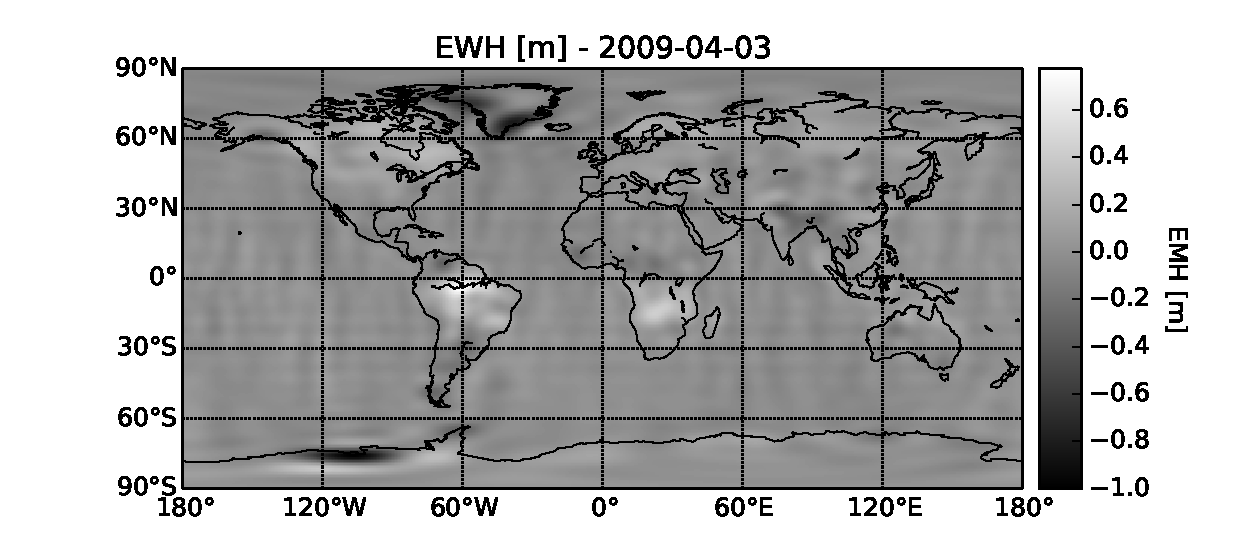
\includegraphics[width=\textwidth]{figures/data-example-world}
	\caption{Plot of the data from 3 April 2009}
	\label{fig:data-example-world}
\end{figure}

\begin{figure}[H]
	\centering
	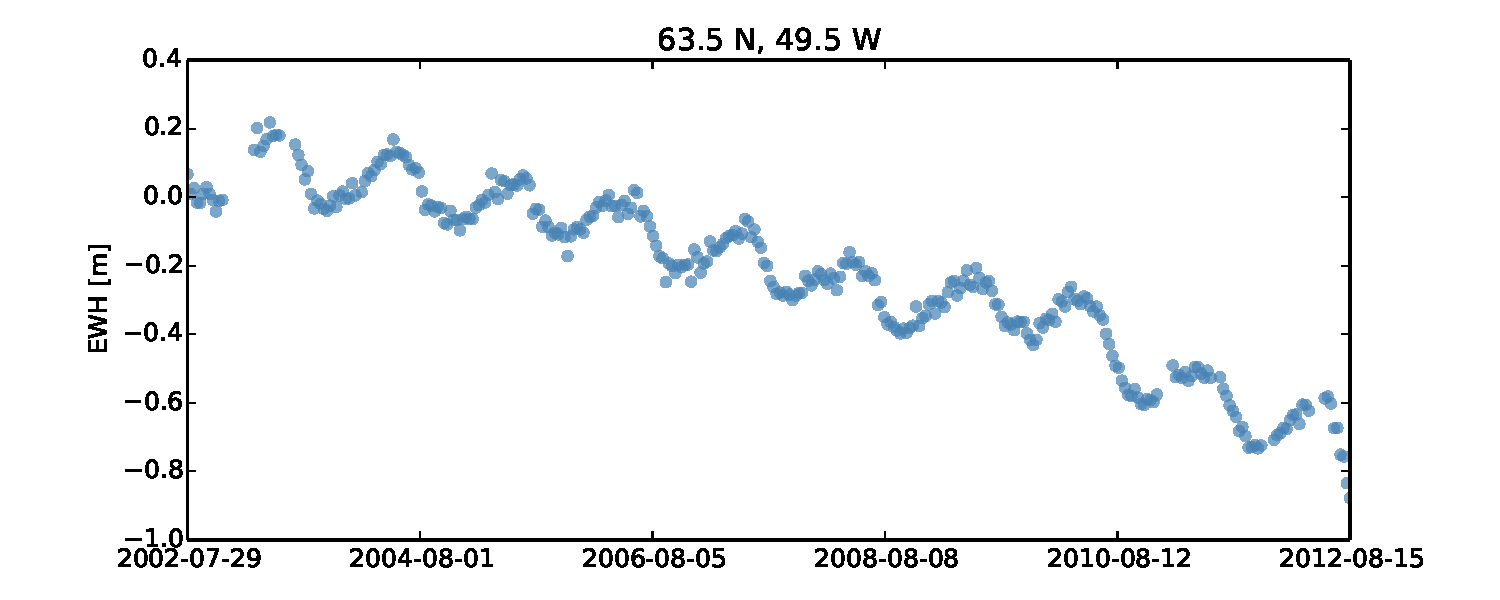
\includegraphics[width=\textwidth]{figures/data-example-scatter}
	\caption{Plot of EWH at 63.5 N 49.5 W, west coast of Greenland.}
	\label{fig:data-example-scatter}
\end{figure}

From Figure \ref{fig:data-example-world} local mass losses at Greenland and the South Pole are seen, this is caused by the ice melting.
A mass increment in South America can also been seen, this is caused by the rain season.
On Figure \ref{fig:data-example-scatter}, mass loss with a yearly periodic trend is seen.


\pagebreak
\section{Theory}
%!TEX root=report.tex
\subsection{SVD}
Singular Value Decomposition (SVD) is a useful method for factorizing matrices.
 According to the SVD-theorem a matrix $X$  can be expressed as
\begin{equation}
X=U \Sigma V^{T}.
\label{eq:theory-svd}
\end{equation}

If the matrix $X$ has the size $m \times n$, the factorized components have the following properties \cite{introduction-to-data-mining}:
\begin{itemize}
\item The columns in $U$ are the eigenvectors of $X X^T$, with the size $m \times m$.
\item The columns in $V$ are the eigenvectors of $X^T X$, with the size $n \times n$.
\item $\Sigma$ is a diagonal matrix, consisting of the square root of the corresponding eigenvalues to the eigenvectors in $U$ and $V$.
It has the size $m \times n$. The square root eigenvalues are also called ``singular values''.
\end{itemize}

In the case where $X$ has many more rows than columns, the $U$ matrix will contain more eigenvectors than are strictly needed to reconstruct $X$ and the $\Sigma$ matrix will have lots of zero-rows.
A so called \textit{economy-size} SVD is therefore often used.
The difference being that all the redundant eigenvectors in $U$ are removed, so it has the size $m \times n$ and the zero-rows from $\Sigma$ are also removed, so its size becomes $n \times n$.

An important property of SVD is that the $V$ matrix contains all eigenvectors and is therefore an orthogonal matrix, for which it is known that
\begin{align}
Q^T = Q^{-1} && Q Q^T = I && Q^T Q = I && \text{, where Q is an orthogonal matrix.}
\end{align}

In the normal SVD (not \textit{economy-size}) $U$ is also a complete orthogonal matrix.
However in \textit{economy-size} some of the columns have been removed, so it is only known that $U^T U = I$.

It is standard procedure to rearrange the matrices in $U \Sigma V^T$, so the largest values in $\Sigma$ appears first in the diagonal.
The reason being that $V$ is a change of basis matrix -- it transforms elements in the original space to a new orthogonal space.
Here the first axis has the largest variance, the second axis has the second highest variance and so on.
The variance described by each axis, is given by the diagonal elements in $\Sigma^2$.
Typically one calculates a percentage called ``variance explained by principal components'' using
\begin{equation}
\rho_{jj} = \frac{\Sigma^2_{jj}}{\sum_{i=1}^n \Sigma^2_{ii}}.
\end{equation}

It is often seen that most of the variance in $X$ can be described using very few eigenvectors, thus one can reduce the dimensionality of a dataset to the most ``principal'' components.
The above mentioned analysis goes under the umbrella term ``Principal Component Analysis (PCA)'', where a ``principal component'' (loadings) should be understood as the axes in the transformed space (i.e., the eigenvectors).

%!TEX root=report.tex
\subsection{OLS}
OLS (Ordinary Least Squares regression) is used for finding the best linear transformations of one or more variables independent $X$ which on average predicts the dependent variable $Y$.
This is done by a matrix-vector product between a $\beta$ vector and $X$.
Since $X$ can be custom tailored for various purposes it is often referred to as the design matrix.

\begin{align}
Y=X \beta +\epsilon && \text{, where } \mathrm{E}[\epsilon] = 0 \text{ and } \mathrm{D}[\epsilon] = \mathrm{D}[Y] = \sigma^2 I .
\end{align}

In the equation above the $\beta$-vector is the unkown parameter which needs to be determined while  $\epsilon$ is a vector containing the variance which the model can't account for (residuals).
Often the purpose of $\beta$ is to propagate predictions of $Y$ for yet unknown $X$-rows, but in this case we want to analyse the individual $\beta_i$ elements.

\subsubsection{The solution to the OLS problem}
As the name eludes, the OLS method minimises the sum of squared residuals ($arg_\beta min \epsilon^T \epsilon$).
It is seen directly that $\epsilon = Y - X \beta$ and thus the following is obtained.

\begin{equation}
\begin{split}
\epsilon^T\epsilon&=(Y-X\beta)^T (Y-X\beta)\\
&=(Y^T-\beta^T X^T) (Y-X\beta) \\
&=Y^T Y-\beta^T X^T Y-Y^T X \beta + \beta^T X^T X \beta \\
&=Y^T Y- 2\beta^T X^T Y+ \beta^T X^T X \beta
\end{split}
\end{equation}

One can now differentiate with respect to the $\beta$ vector.
\begin{equation}
\begin{split}
\frac{\partial \epsilon^T\epsilon}{\partial \beta}&=-2 X^T Y+2X^T X \beta=2(-X^T Y+X^T X \beta).
\end{split}
\end{equation}

Now  $\epsilon^T \epsilon$'s minimum is given by solving for $\frac{\partial \epsilon^T\epsilon}{\partial \beta} = 0$
\begin{equation}
\begin{split}
\frac{\partial \epsilon^T\epsilon}{\partial \beta} = 0 \Rightarrow 2(-X^T Y+X^T X \hat{\beta}) &= 0 \\
X^T X \hat{\beta}&=X^T Y \\
\hat{\beta}&=(X^T X)^{-1} X^T Y.
\end{split}
\end{equation}

The solution above is formally correct \cite[s.~12]{statistical-learning}, but if $X$ is badly conditioned $(X^T X)^{-1}$ might not be numerically stable (i.e. if the columns in $X$ are highly correlated leading to a near singular $X$).\todo{kilde, husker det er enten Henrik eller Allan}
To avoid this problem $X$ should be factorised and the solution reformulated; in this report we will exclusively do this using SVD.
\begin{equation}
\begin{split}
\hat{\beta} &= (X^T X)^{-1} X^T Y \\
&= \left( \left(U \Sigma V^T\right)^T \left(U \Sigma V^T\right) \right)^{-1} \left(U \Sigma V^T \right)^T Y \\
&= \left( V \Sigma^2 V^T \right)^{-1} \left(U \Sigma V^T \right)^T Y \\
&= V \Sigma^{-1} U^T Y.
\end{split}
\end{equation}

It should be noted, that when multiple $\beta$ vector needs to be calculated (one vector for each spatial location on the surface) further optimizations are possible.
By arranging $Y$ as a matrix with each column corresponding to a location, $\beta$ will be a matrix containing all solutions instead of a vector containing only one solution.

\subsubsection{The ``Hat" matrix}
In the special case of the GRACE data, the $X$ matrix (containing the time of measurements and transformations of the time) is identical for every position. This can be exploited by constructing a hat matrix$H$ which only depends on $X$ and projects $Y$ onto $\hat{Y}$ (puts the hat on $Y$).
\begin{equation}
\begin{split}
\hat{Y} &= X \hat{\beta} \Rightarrow \hat{Y} = X V \Sigma^{-1} U^T Y \\
\hat{Y} &= H X \quad \text{, hvor } H = X V \Sigma^{-1} U^T.
\end{split}
\end{equation}

As earlier with $\beta$, the hat matrix can be calculated for all $Y$ vectors by horizontally stacking $Y$s to form a matrix.

An important propoerty of the $H$ matrix is that it is idempotent ($H^2 = H$).
Remember that $H$ was a projection matrix which projected $Y$ onto $\hat{Y}$.
So if one were to project $Y$ onto $\hat{Y}$ and then project again, of course nothing happens because one is already in the $\hat{Y}$-plane.

\subsubsection{Root Mean Squared Error}

``Root Mean Squared Residuals'' (RMSE) is an indicator of how good an $Y$ estimate is.
It can be calculated as
\begin{equation}
\hat{\sigma} = \sqrt{\frac{\left(Y - \hat{Y}\right)^T \left(Y - \hat{Y}\right)}{N-p}},
\end{equation}

where $p$ is the number of parameters (elements in $\beta$) and $N$ is the number of observations (elements in $Y$).
RMSE is an estimate for the standard deviation of $Y$ \cite[theorem~3.4]{time-series-analysis} thus the symbol $\hat{\sigma}$.


\subsubsection{The variance of $\hat{Y}$}

The dispersion (variance-covariance) of $\hat{Y}$ can be calculated as
\begin{equation}
\mathrm{D}[\hat{Y}] = \mathrm{D}[H Y] = H \mathrm{D}[Y] H^T = \sigma^2 H^2 = \sigma^2 H
\end{equation}

The variance of $\hat{Y_i}$ is given by the diagonal elements ini $\mathrm{D}[\hat{Y}]$:
\begin{equation}
\mathrm{Var}[\hat{Y_i}] = \sigma^2 diag(H_{ii})
\end{equation}

Because $\sigma^2$ is a scalar, the diagonal in $H$ is important to examine, since it can reveal potentiel elements (in our case points of time) with high variance in the predictions.

\subsubsection{The dispersion of $\hat{\beta}$}

The dispersion of $\hat{\beta}$ is calculated as \cite[theorem~3.2]{time-series-analysis}:
\begin{equation}
\mathrm{D}[\hat{\beta}] = \sigma^2 (X^T X)^{-1} = \sigma^2 V \Sigma^{-2} V^T
\end{equation}

Seeing as $\sigma^2$ is a scalar and dependent of $Y$, the expression can be made independent of position (because of identical $X$ matrices) by looking exclusively at $V \Sigma^{-2} V^T$.


\subsubsection{P-values for $\hat{\beta}$}

To calculate p-values for OLS parameters we assume that they follow the student's t-distribution and thus firstly need to calculate the t-value \cite{t-value-ols}:
\begin{align}
\mathrm{t} = \frac{\beta_i}{\mathrm{SD}[\beta_i]} && \text{hvor: } \mathrm{SD}[\beta_i] = \sqrt{\mathrm{Cov}[\hat{\beta}]_{ii}} = \hat{\sigma} \sqrt{ (V \Sigma^{-2} V^T)_{ii} }
\end{align}

Now by plucking the t-value into the CDF ``student's t cumulative distribution function'' ($\Phi_t$) , and adjusting the degrees of freedom to $N - p$ we get
\begin{equation}
p = \Phi_t\left(\mathrm{t}, N-p\right)
\end{equation}

The null-hypothesis is that $\beta_i = 0$ and the alternate hypothesis is $\beta_i \not = 0$.


%!TEX root=report.tex
\subsection{Design matricen $X$}
Design matricen er $X$ matrix i OLS regression, hvis kolonner indgå i en linear kombination til at beskrive $Y$.
I tilfældet for GRACE data er de eneste ``$x$'' værdier tiden ($\mathbf{t}$), og som udgangspunkt vil $X$ derfor have formatet:
\begin{equation}
X = \left[\begin{matrix} \mathbf{1} & \mathbf{t} \end{matrix}\right].
\end{equation} 
Dette vil betyde at $\hat{Y}$ skal beskrives som $\beta_1 + \beta_2 t$, hvor $\beta_1$ vil være startværdien (uinteressant) og $\beta_2$ vil være hastigheden i udviklingen.
Det fremkommer således naturligt at også have accelerationen i udviklingen med:
\begin{equation}
X = \left[\begin{matrix} \mathbf{1} & \mathbf{t} & \frac{1}{2} \mathbf{t}^2 \end{matrix}\right]
\end{equation} 

Fra Fourier analyse vides det, at funktioner kan anproximeres en uendelige sum af sinus og cosinus funktioner.
Disse trigonometriske funktioner er periodiske og kan således indeholde periodiske signaler, der måtte forkomme i den funktion, man ønsker at approximere.

I GRACE datasættet er der dog ikke en uendelig lille afstand (i tiden) imellem målingerne, en uendelig række af sinus og cosinus funktioner benyttes derfor ikke.
I stedet antages det, at den største forekommende svingning er en årssvingning ($365.242$ dage).
Den mindste svingning(frekvens) som man kan observere når man sampler et signal er Nyquist frekvensen.
I GRACE tilfældet er der 10 dage imellem hver måling, Nyquist frekvensen bliver så $\frac{1}{2 \cdot 10} = \sfrac{1}{20}$ dage.
Dette svarer ca til 18 svingninger pr. år da $\sfrac{365.242}{18} \approx 20.29$. Således fås den endelige design matrix
\begin{equation*}
\resizebox{\textwidth}{!}{$
X = \left[\begin{matrix}
	\mathbf{1} &
	\mathbf{t} &
	\frac{1}{2} \mathbf{t}^2 &
	\cos\left( \frac{2 \pi}{\frac{365.242}{1}} \mathbf{t} \right) &
	\sin\left( \frac{2 \pi}{\frac{365.242}{1}} \mathbf{t} \right) &
	\cdots &
	\cos\left( \frac{2 \pi}{\frac{365.242}{18}} \mathbf{t} \right) &
	\sin\left( \frac{2 \pi}{\frac{365.242}{18}} \mathbf{t} \right)
\end{matrix}\right].
$}
\end{equation*}


%!TEX root=report.tex
\subsection{Phase and Amplitude}

The $\mathbf{\beta}$ parameters in the OLS problem are linear combinations of $\cos(\omega_i t)$ and $\sin(\omega_i t)$ function pairs.
However from a physics perspective having both $\cos(\omega_i t)$ and $\sin(\omega_i t)$ for the same $\omega_i$ have no meaning.
Instead one should convert the $\beta$ parameters for the trigonomic functions intro amplitude and phase for a single periodic function $A_i \cos(\omega_i t + \phi_i)$.
This is done by using Ptolemy's theorem
\begin{equation}
A_i \cos(\omega_i t + \phi_i) = A_i \cos(\phi_i) \cos(\omega_i t) - A_i \sin(\phi_i) \sin(\omega_i t).
\end{equation}

Comparing with the linear combination from OLS
\begin{align}
\hat{Y} = \cdots + \beta_{c,i} \cos(\omega) + \beta_{s,i} \sin(\omega) + \cdots
\end{align}
it's see that
\begin{align}
\beta_{c,i} = A \cos(\phi_i) && \text{ and } && \beta_{s,i} = A \sin(\phi_i).
\end{align}

By dividing these two equations with each other, $\phi_i$ can be calculated as \todo{This is not the one used in the code. (Sign diffrence)} 
\begin{equation}
\frac{- A_i \sin(\phi_i)}{A_i \cos(\phi_i)} = \frac{\beta_{s,i}}{\beta_{c,i}} \Rightarrow \phi_i = \arctan\left(-\frac{\beta_{s,i}}{\beta_{c,i}}\right).
\end{equation}

To isolate $A_i$, square both equations and add them together:
\begin{equation}
A_i^2 \cos(\phi_i)^2 + A_i^2 \sin(\phi_i)^2 = \beta_{c,i}^2 + \beta_{s,i}^2 \Rightarrow A_i = \sqrt{\beta_{c,i}^2 + \beta_{s,i}^2}.
\end{equation}

The result can be plotted with a circular color scale for the $\phi_i$ and $A$ is then the intensity of the color.

%!TEX root=report.tex
\subsection{Least angular regression and shrinkage (LARS)}
We'll here briefly discuss the LARS model.
It's almost equivalent to the linear regression, except that instead of only minimizing the sum of squares, a L1-norm penalty as added on the $\beta$-vectors coefficients.
\begin{equation}
MIN: (Y-\hat{Y}).T (Y-\hat{Y}) | \{||\beta||_1<s\}
\end{equation}

The LARS algorithm \footnote{source:statweb.stanford.edu/~tibs/lasso/simple.html} solves this problem by initially letting all the $\beta$ coeffients be zero.
It then finds the attribute,$b_1$ with the highest absolute correlation with y and increases (or decreases depending on the sign of the correlation)
until it reaches a point where another attribute $b_2$ has as much  correlation with the residuals $R=Y-\hat{Y}$ as  $b_i$ has.
At this point the algorithm then increases both $b_1$ and $b_2$ in their join direction until another attribute $b_i$ has the highest residual correlation.
This process can then be continued until there is no benefit in increasing any of the $b_i$s - that is the full LARS solution is equivalent to the linear regression.
It should also be noted that if a coefficient crosses 0 in a iteration (step),
that the coefficient should be set to 0, and the regression direction should subsequently be recomputed.

So why might one use LARS instead of for example LASSO model with a specific $alpha$?
Well in the LARS model you actually get the full solution path which means that you can find all the lasso solutions.


\section{Resultater}
%!TEX root=report.tex

\subsection{time series analysis - ARIMA}

To get an indication if its possible to use time series analysis on the GRACE data, a single position (63.5 N 49.5 W, west coast of Greenland) have been selected.

To analyze the data using an ARIMA model an equidistant dataset is required. For example it would otherwise not possible to solve the Yule-Walker equations \cite[s.~122]{time-series-analysis}. In the original GRACE dataset some values are missing, thus they should be interpolated. Also in order to get an indication of the model performance, the last 36 observations (a year) have been separated for cross validation testing.

\begin{figure}[H]
\centering
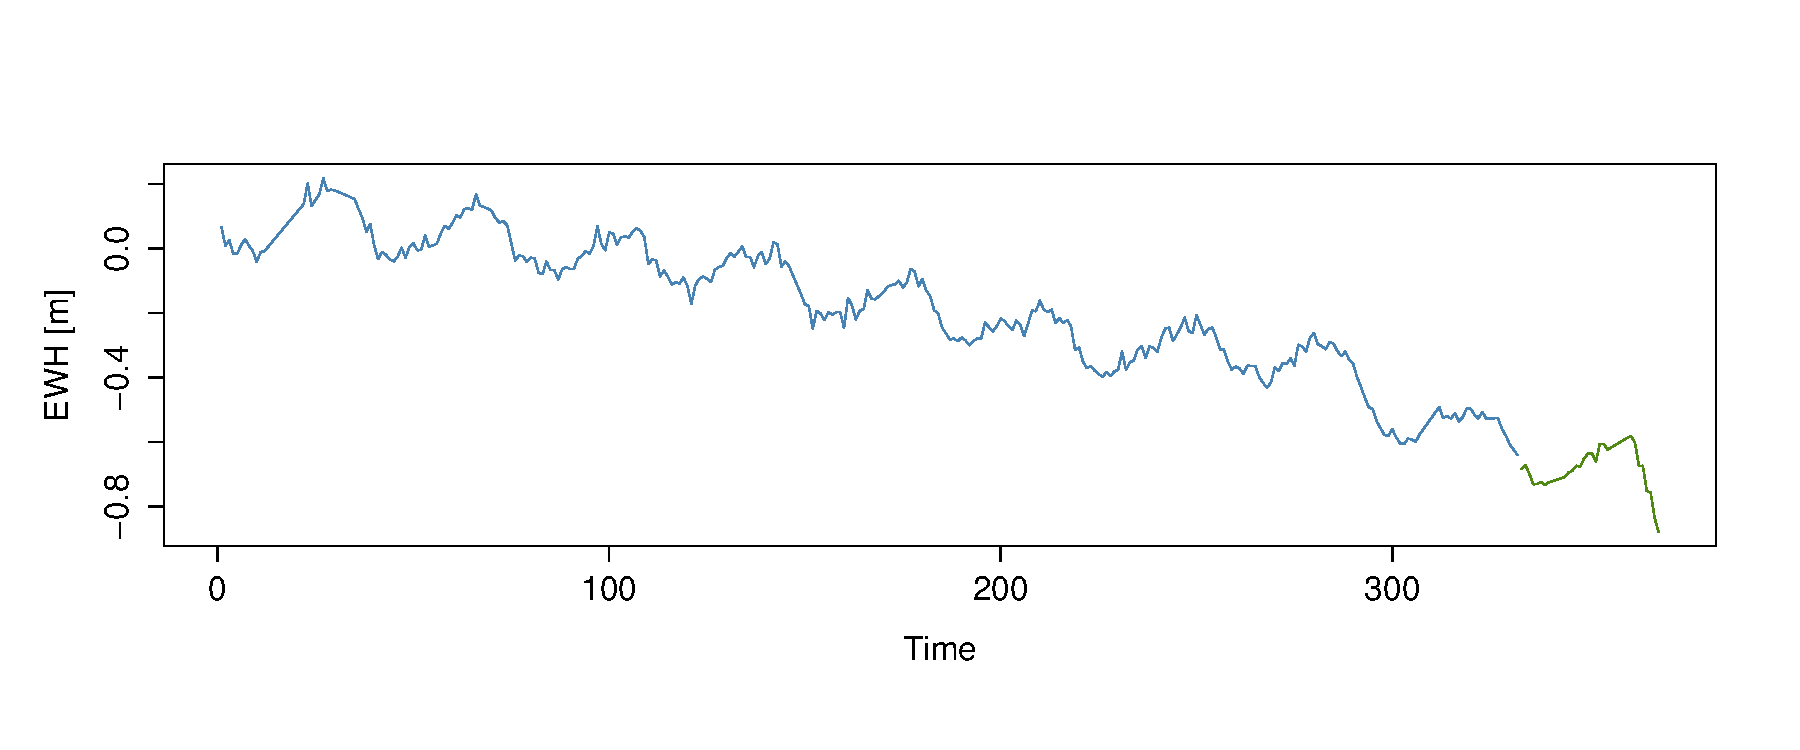
\includegraphics[height=5cm]{figures/ts-initial-split}
\caption{GRACE data at 63.5 N 49.5 W, where missing values are interpolated. Blue is the training data and green is the  test data.}
\label{fig:ts-initial-split}
\end{figure}

The time series in Figure \ref{fig:ts-initial-split} is clearly not stationary, thus it is necessary to consider the time series difference.
\begin{figure}[H]
\centering
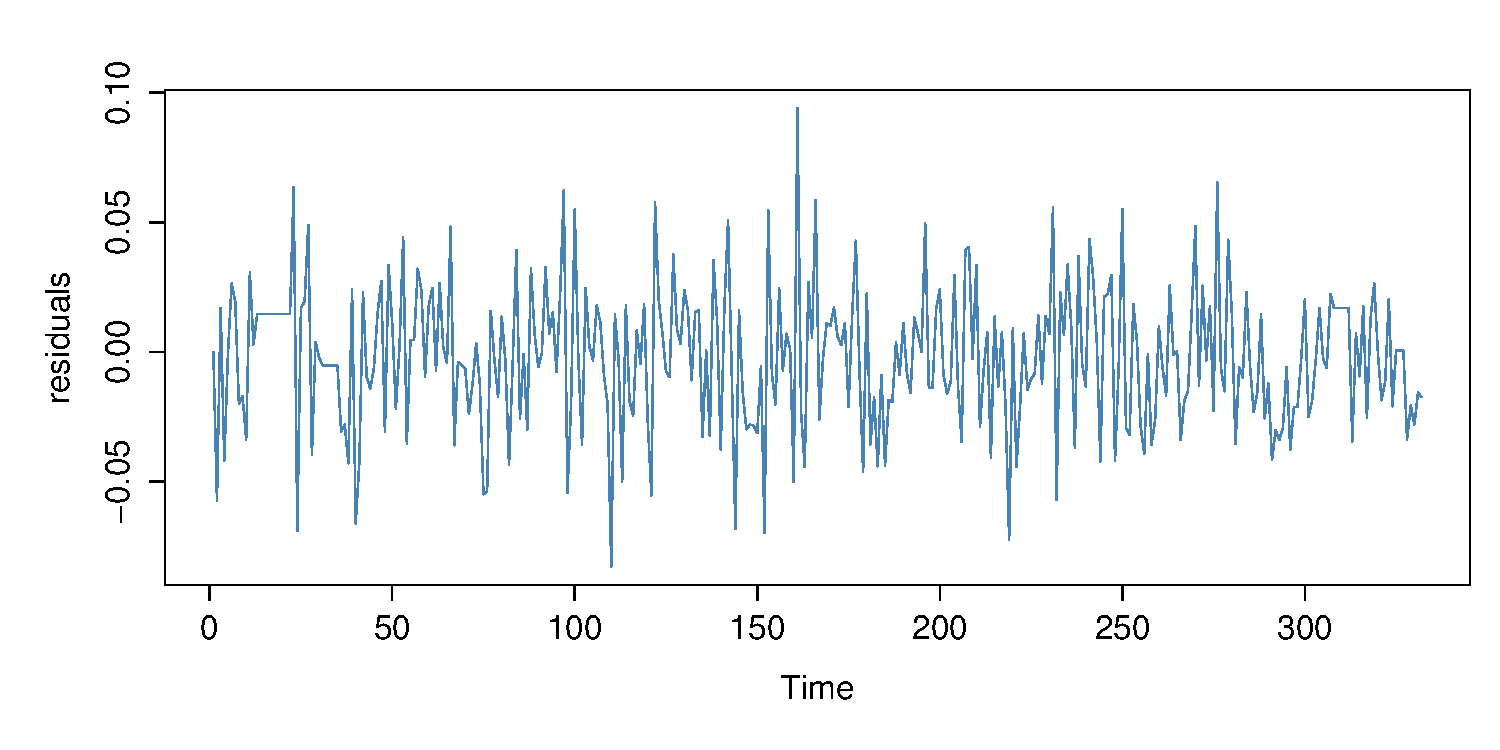
\includegraphics[height=5cm]{figures/ts-residual-i1s0}
\caption{The ARIMA$(0,1,0) \times (0,0,0)_{36}$ residuals.}
\label{fig:ts-residual-i1s0}
\end{figure}
On Figure \ref{fig:ts-residual-i1s0} there some seasonal periods where the mean and variance isn't the same as the remaining period, thus it is not completely stationary. Taking also the seasonal difference (assuming the season is 36 observations, a year) gives however a very stationary output.

\begin{figure}[H]
\centering
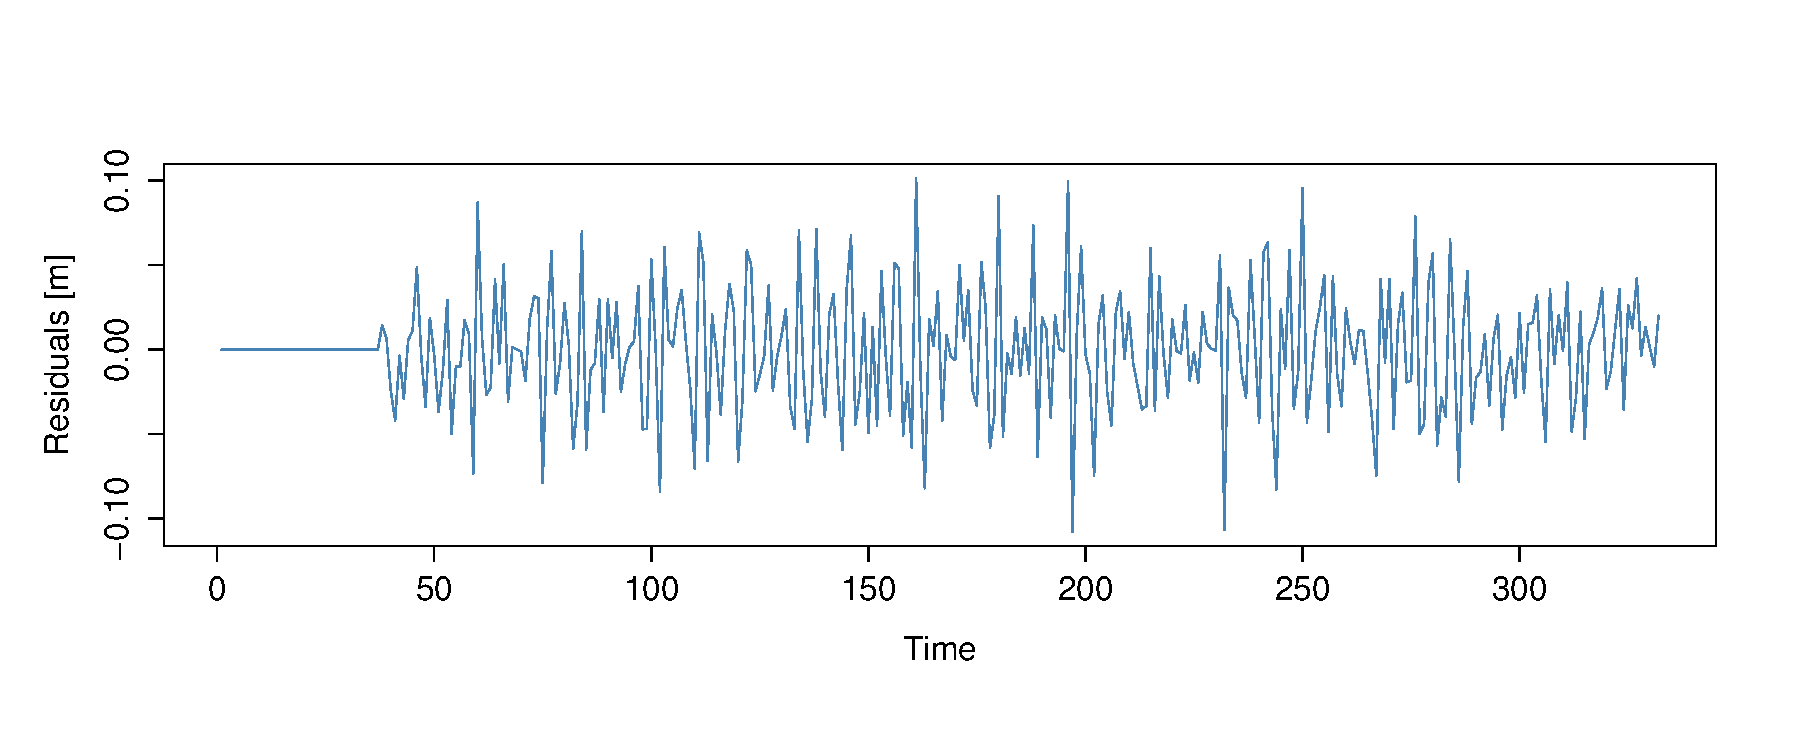
\includegraphics[height=5cm]{figures/ts-residual-i1s1}
\caption{The ARIMA$(0,1,0) \times (0,1,0)_{36}$ residuals.}
\label{fig:ts-residual-i1s1}
\end{figure}
On Figure \ref{fig:ts-residual-i1s1} its seen that the first 37 observations acts strange, this is because there aren't enough past observations to estimate the EWH correctly, thus they should be excluded from further analysis.

To determine the AR and MA terms in the ARIMA mode, the ACF and PACF should be estimated using the residuals from Figure \ref{fig:ts-residual-i1s1}.
\begin{figure}[H]
	\centering
	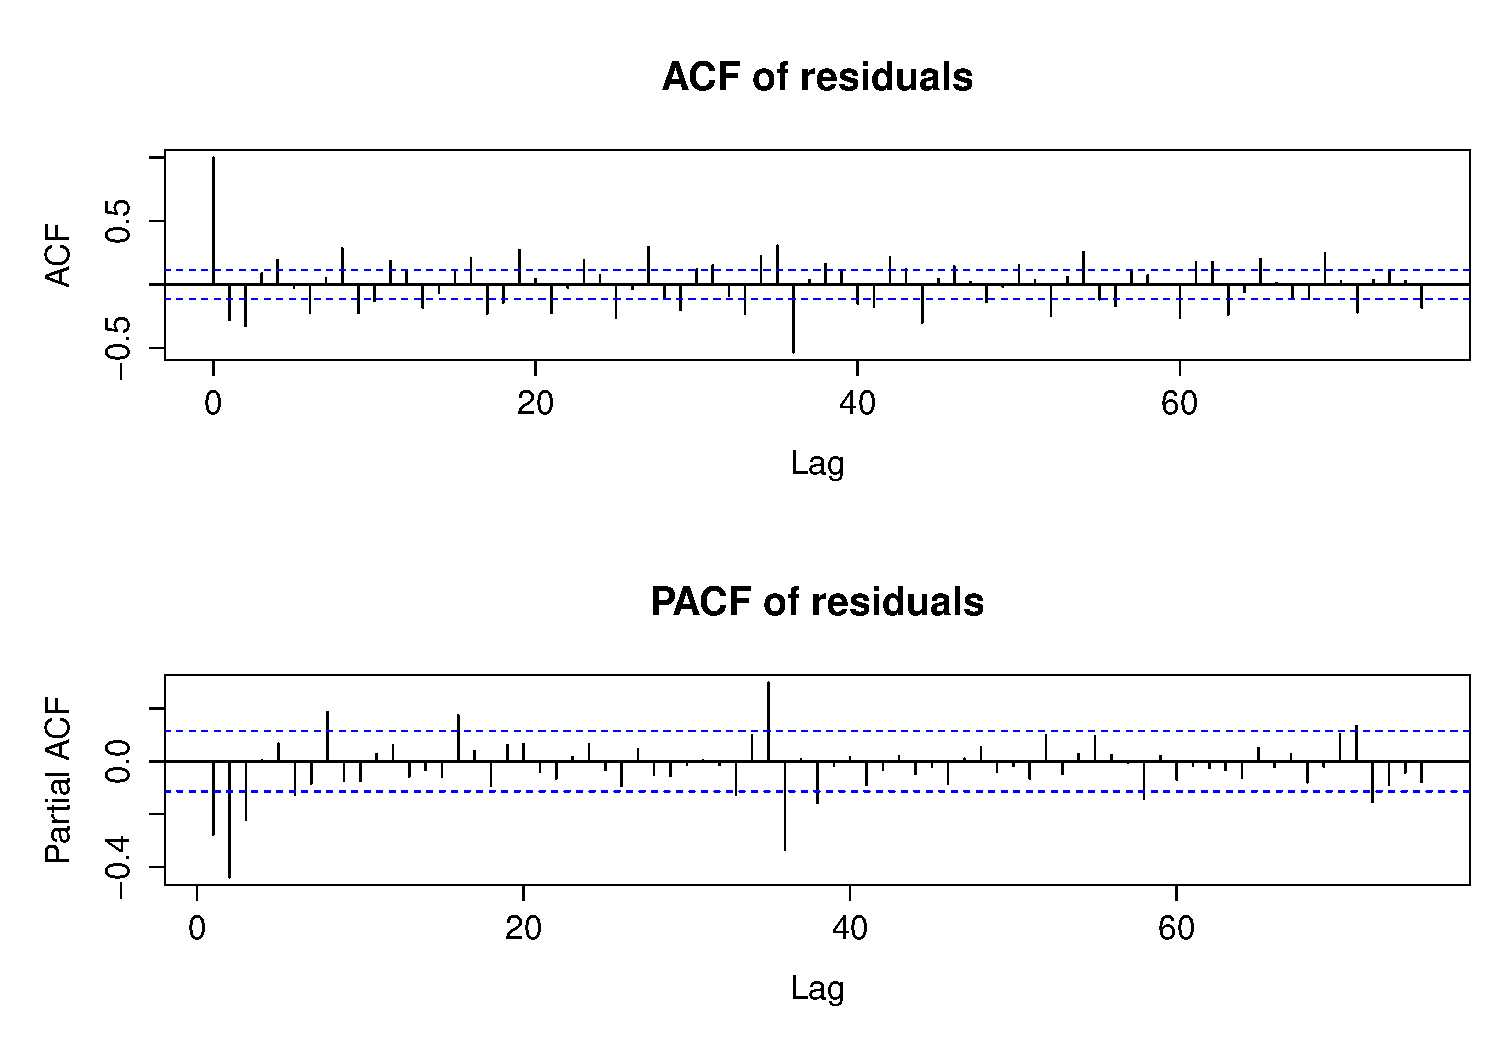
\includegraphics[width=\textwidth]{figures/ts-acf-ar0s0}
	\caption{ACF and PACF for ARIMA$(0,1,0) \times (0,1,0)_{36}$ residuals}
	\label{fig:ts-acf-ar0s0}
\end{figure}

Using the PACF in Figure \ref{fig:ts-acf-ar0s0} and the rules for the AR term \cite[Table~6.1]{time-series-analysis} \texttt{AR(2)}, seams like a good guess for the non-seasonal AR term.
\begin{figure}[H]
	\centering
	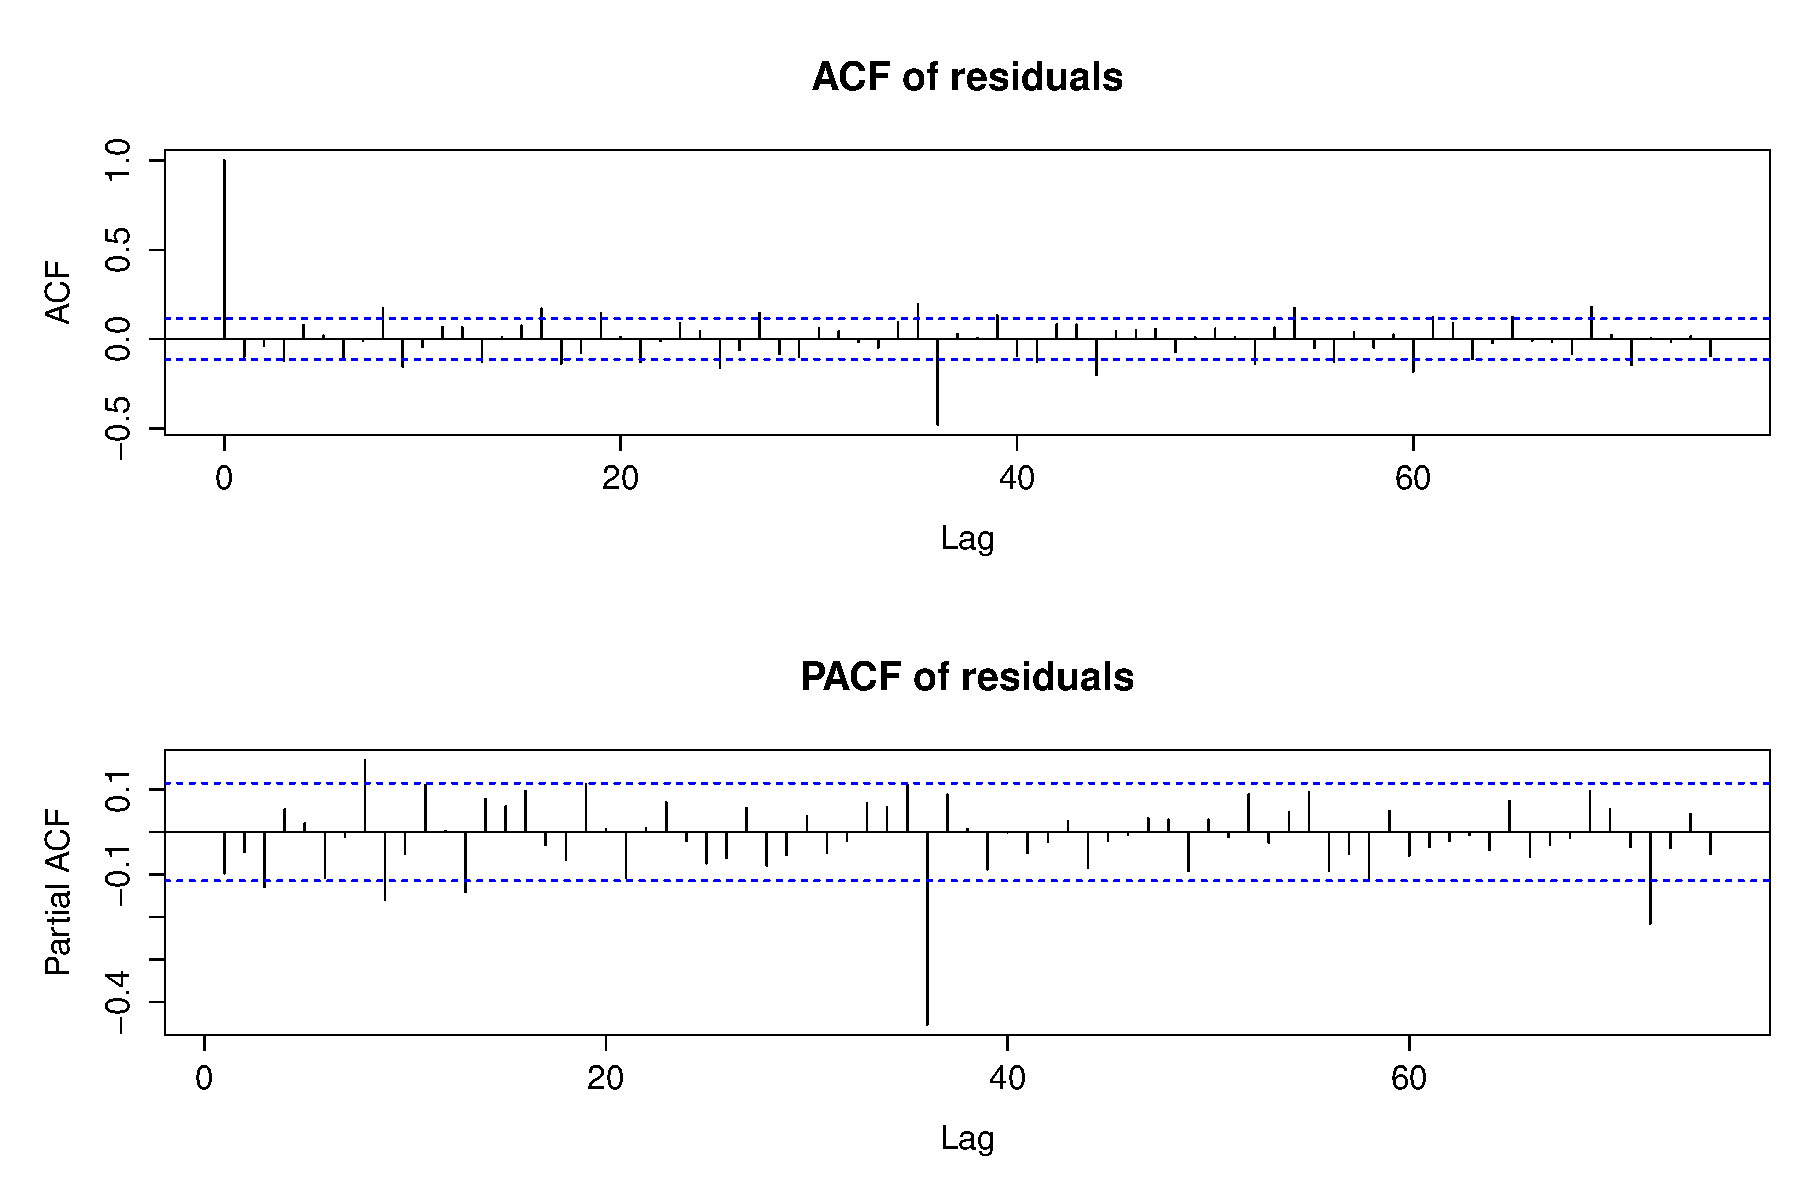
\includegraphics[width=\textwidth]{figures/ts-acf-ar2s0}
	\caption{ACF and PACF for ARIMA$(2,1,0) \times (0,1,0)_{36}$ residuals}
	\label{fig:ts-acf-ar2s0}
\end{figure}

This clearly fitted the non-seasonal trend. From Figure \ref{fig:ts-acf-ar0s0} it might have looked like there was a \texttt{AR(3)} or \texttt{MA(2)} term, but the \texttt{AR(2)} is the simplest of those and fit the trend just fine. The seasonal part is now extremely apparent in Figure \ref{fig:ts-acf-ar2s0}, where it looks like either an \texttt{SAR(2)}.
\begin{figure}[H]
	\centering
	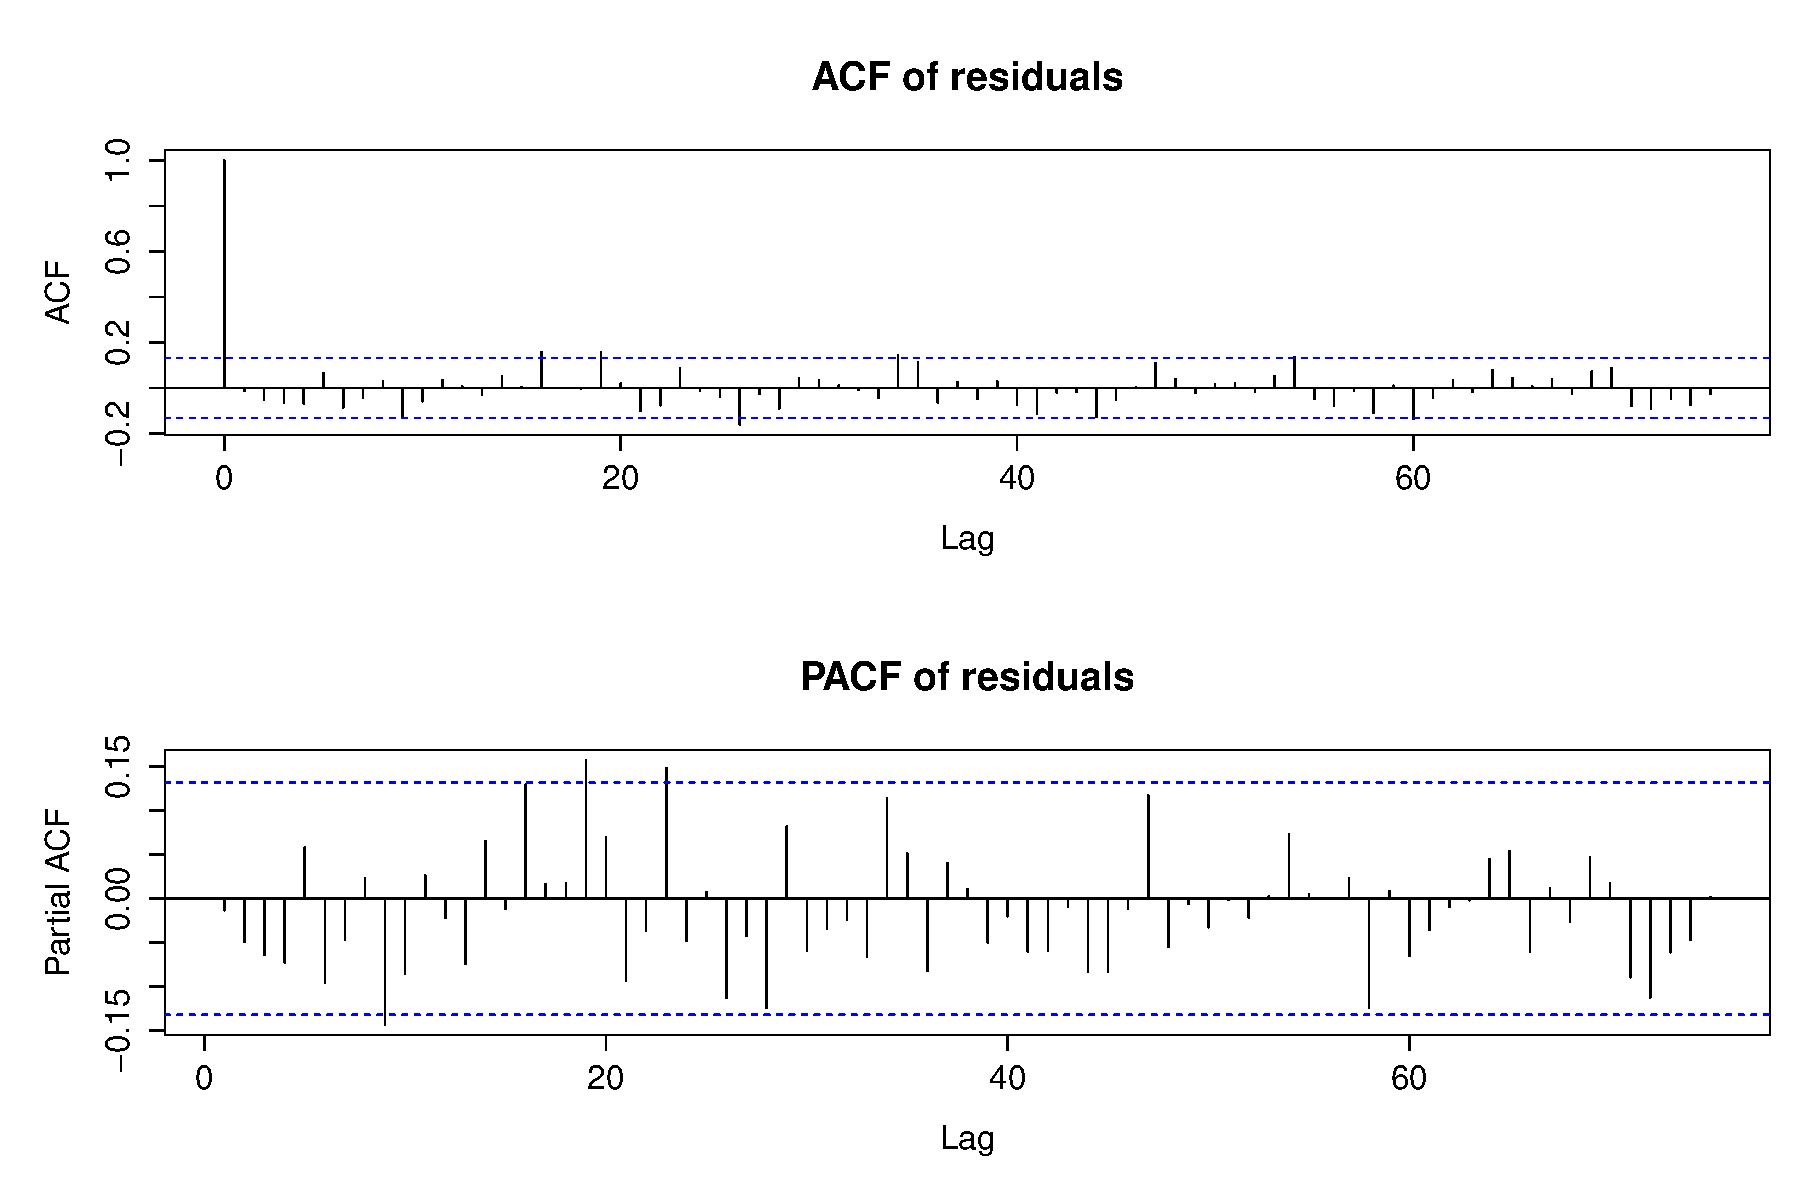
\includegraphics[width=\textwidth]{figures/ts-acf-ar2s2}
	\caption{ACF and PACF for ARIMA$(2,1,0) \times (2,1,0)_{36}$ residuals}
	\label{fig:ts-acf-ar2s2}
\end{figure}

From just looking at the estimated ACF and PACF in Figure \ref{fig:ts-acf-ar2s2}, ARIMA$(2,1,0) \times (2,1,0)_{36}$ seams like a good choice. To finally validate the model, a good start is to look at the residuals.
\begin{figure}[H]
	\centering
	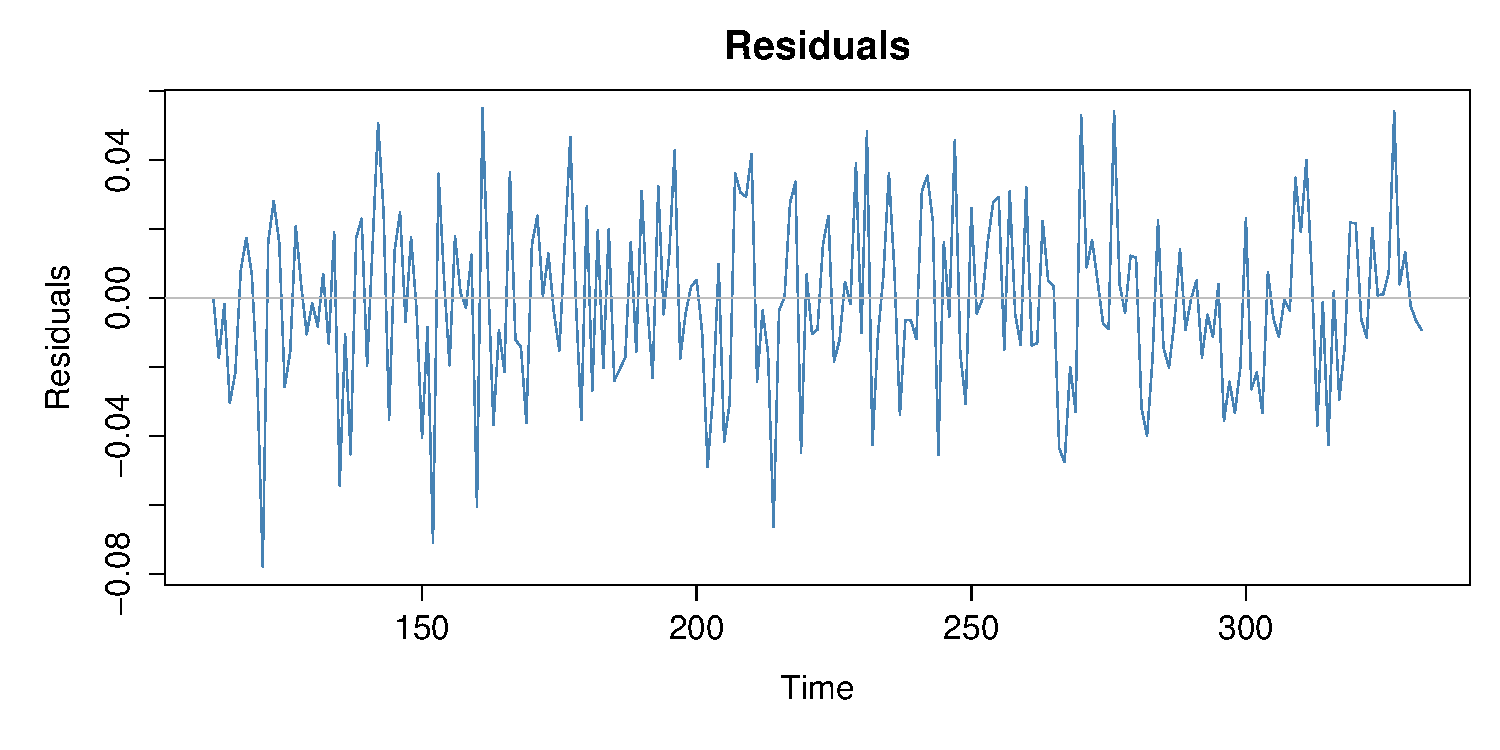
\includegraphics[height=5cm]{figures/ts-final-residual}
	\caption{ARIMA$(2,1,0) \times (2,1,0)_{36}$ residuals. The first 111 residuals have been skipped since they can't be estimated correctly.}
	\label{fig:ts-final-residual}
\end{figure}

Figure \ref{fig:ts-final-residual} looks stationary, there are no outliers nor seasonal trends. To validate the model further the Ljung-Box test can be used. This however requires the residuals to be normally distributed, a QQ-plot (Figure \ref{fig:ts-final-qq}) shows that this is the case:
\begin{figure}[H]
	\centering
	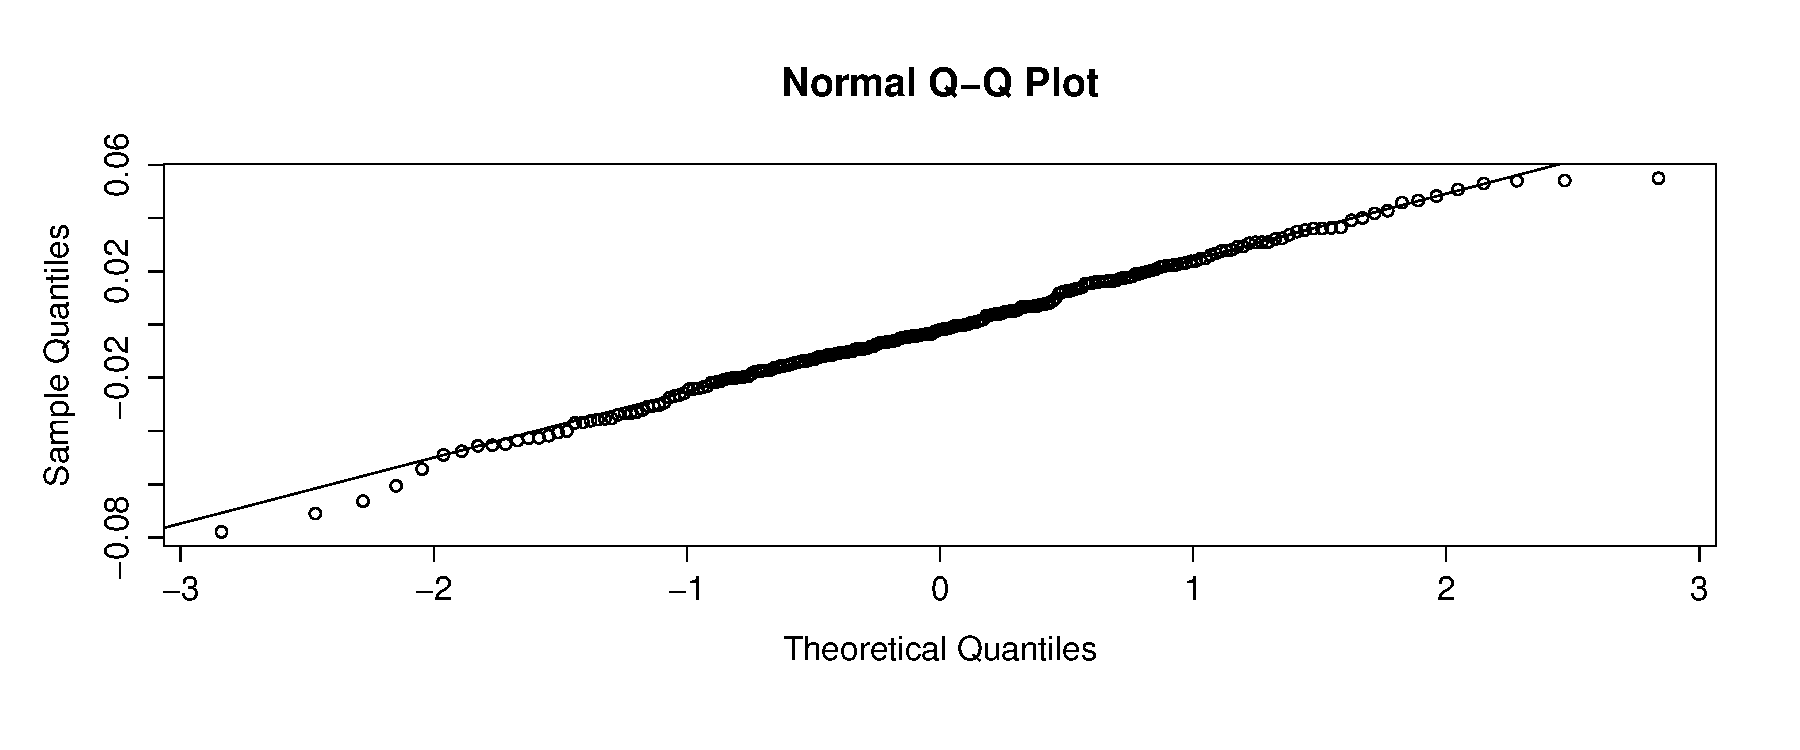
\includegraphics[height=5cm]{figures/ts-final-qq}
	\caption{QQ-plot for the ARIMA$(2,1,0) \times (2,1,0)_{36}$ residuals.}
	\label{fig:ts-final-qq}
\end{figure}

\begin{figure}[H]
	\centering
	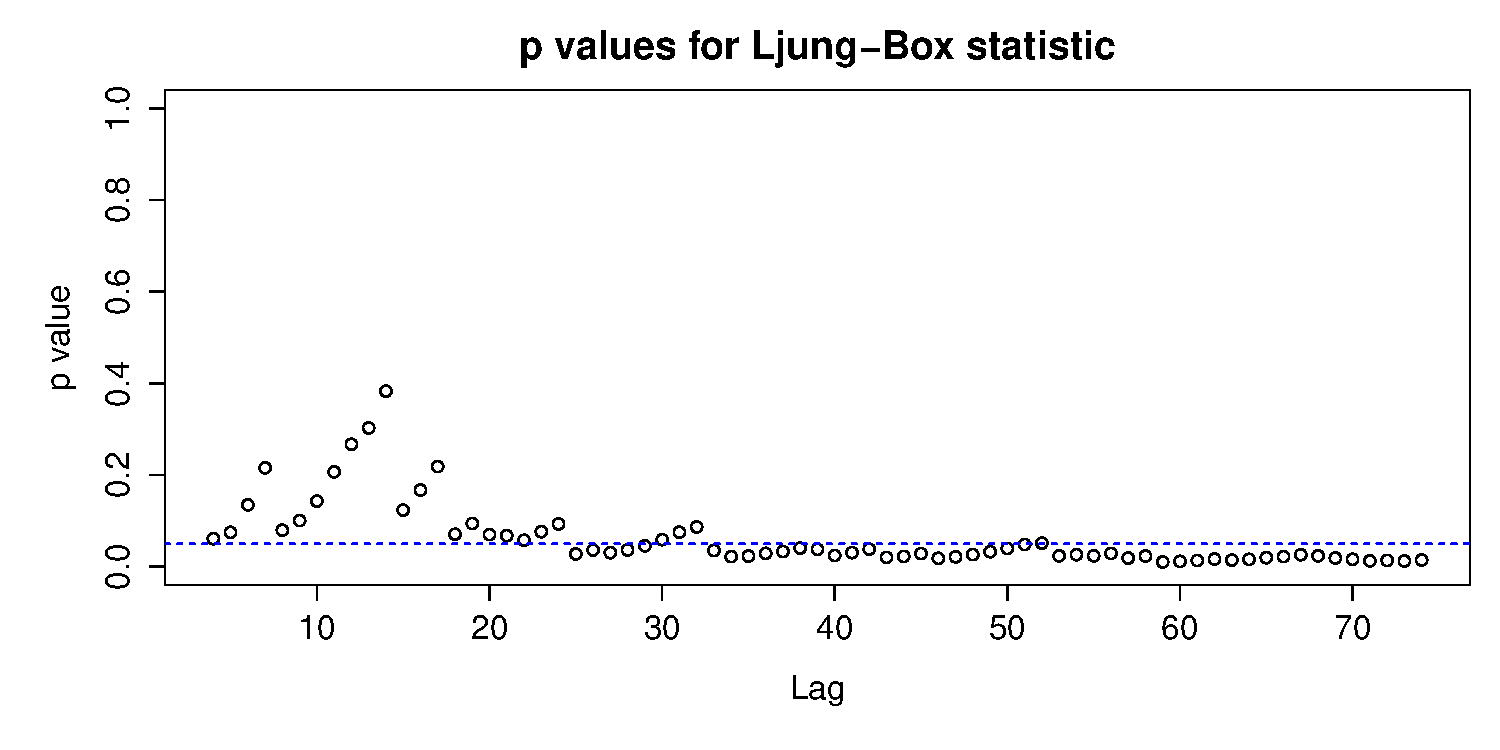
\includegraphics[height=5cm]{figures/ts-final-ljungbox}
	\caption{Ljung-Box test for the ARIMA$(2,1,0) \times (2,1,0)_{36}$ residuals.}
	\label{fig:ts-final-ljungbox}
\end{figure}

From the Ljung-Box test (Figure \ref{fig:ts-final-ljungbox}) the p-value for the first many lags looks good, however after 25 it can be with 95\% confidence statically significant concluded that the residuals are correlated. In terms of pure time series analysis is makes the model quite useless, however it is still valuable to do the cross validation.

\begin{figure}[H]
\centering
\centerline{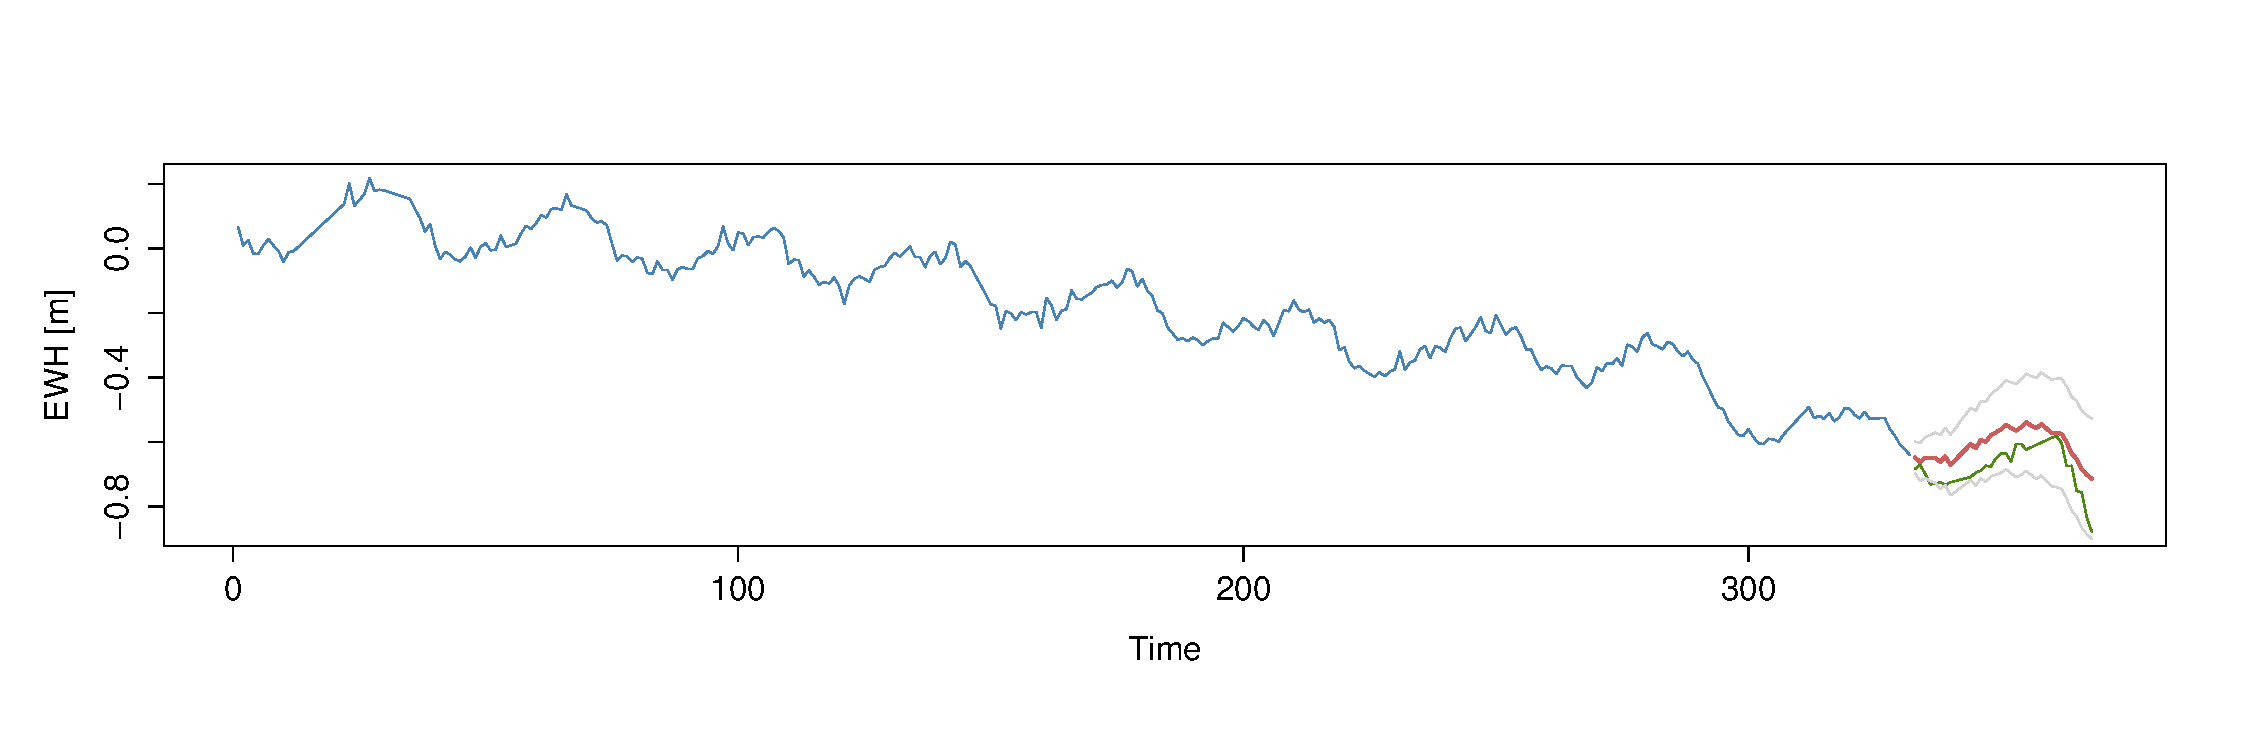
\includegraphics[height=5cm]{figures/ts-final-forecast}}
\caption{Forecast on Cross Validation. Blue is the training data, green is the test data. Red is then the predicted test values with its 95\% confidence interval marked with gray lines.}
\label{fig:ts-final-forecast}
\end{figure}

From Figure \ref{fig:ts-final-forecast} it quite clear that the test data is consistently bellow the expectation line (red). While it is still inside the 95\% confidence interval, this high correlation in the error between lags indicates that the model isn't particular useful. 

%!TEX root=report.tex
\pagebreak
\subsection{LARS}

Below the full solution path of all the 39 coefficients is shown.
\begin{figure}[H]
\center
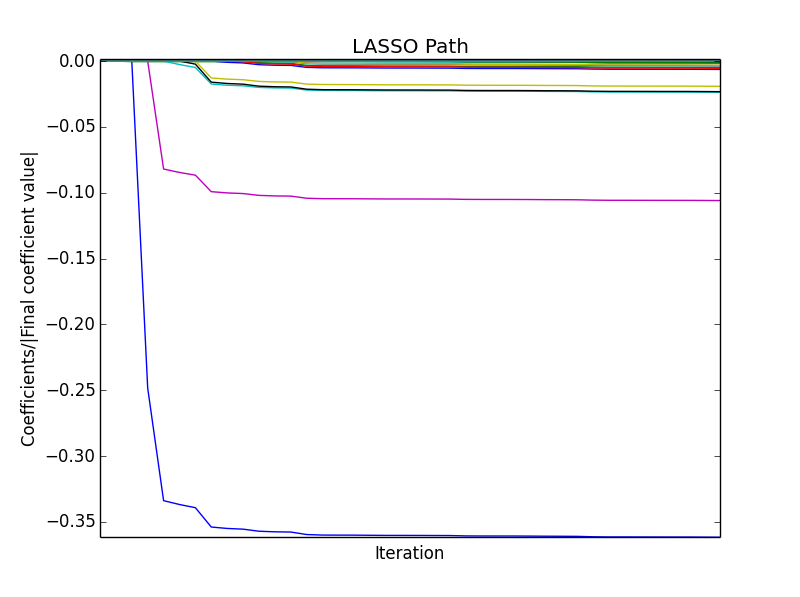
\includegraphics[width=10cm]{figures/lasso_path.png}
\caption{The above plot illustrates the coefficient path, for the solution corresponding to a point on the west coast of Greenland (coordinates [24,134]).}
\end{figure}
In the above plot it appears that after iteration 7 the coefficients doesn't really change that much. However since the lines are a bit to entangled to inspect visually, one can also plot the coefficent value divided by the final coefficient value, on the y axis:
\begin{figure}[H]
\center
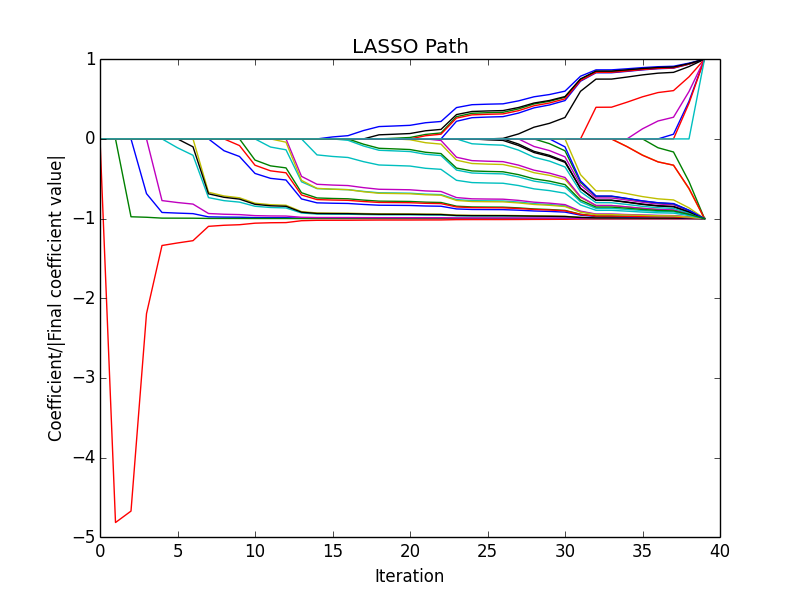
\includegraphics[width=8cm]{figures/lasso_path_scaled.png}
\caption{Scaled coefficients}
\end{figure}
\pagebreak
The 7 chosen coefficients and their values are :
\begin{lstlisting}[mathescape]

[ -3.53905876e-01  -4.28123366e-04  -1.13665156e-07  -1.74354380e-02  -9.91803076e-02  -1.28215596e-02  -1.60040198e-02]

[intercept (1), slope (t), acc. ($0.5  t^2$),$ cos(\frac{2\pi}{365.2 }t)$, $sin(\frac{2\pi}{365.2  }t)$, $cos( \frac{2\pi}{182.6  }t)$, $sin(\frac{2\pi}{182.6* t})$]
\end{lstlisting}
Using these 7 coefficients we get the following results:
\begin{figure}[H]
\center
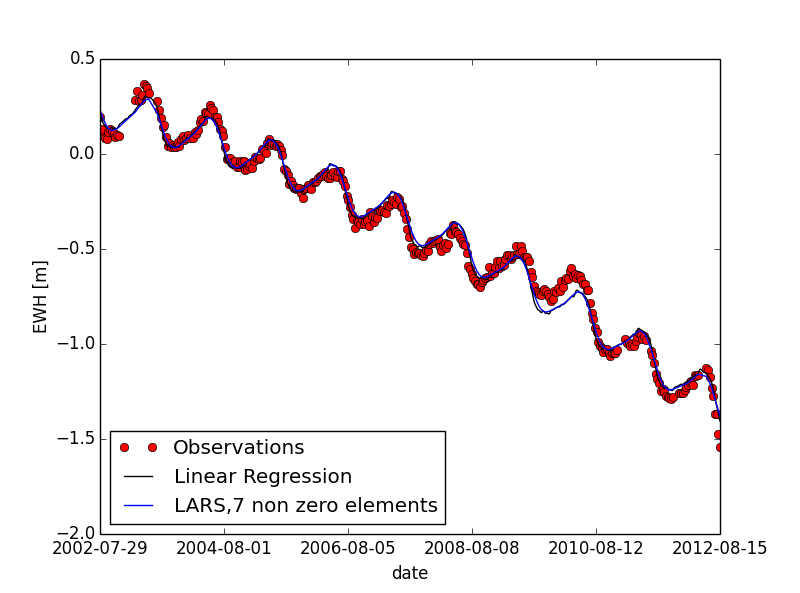
\includegraphics[width=10cm]{figures/lars_7.png}
\caption{It's evident from the graph that the LARS solution is very similar to the linear regression.}
\end{figure}

\subsubsection{How many frequencies are actually needed}

Ofcourse since this was only done for 1 point on the globe, if one were to apply this to other points one might get different lasso-paths and perhaps also a slight variance in the amount of coefficients needed. For example for modelling the ocean one wouldn't need as many coefficients, while potentially at places with heavy rain season, such as South America you might need more frequencies.


\pagebreak
%!TEX root=report.tex
\section{Appendix}


\subsection{Tidsrækkeanalyse resultater}
\label{first-R}

Den første model baseret på graf-aflæsninger (R-output):

\begin{minipage}{1.3\textwidth}
\begin{lstlisting}
Series: xdata 
ARIMA(3,1,3)(1,1,4)[36]                    

Coefficients:
          ar1     ar2     ar3     ma1      ma2     ma3    sar1     sma1    sma2
      -0.3860  0.1239  0.0471  0.2225  -0.2783  0.0035  0.0926  -0.9147  0.1808
s.e.   0.1556     NaN     NaN  0.1673      NaN     NaN     NaN      NaN  0.0508
        sma3     sma4
      0.0980  -0.1206
s.e.  0.0466   0.0749

sigma^2 estimated as 0.0005546:  log likelihood=727.89
AIC=-1431.78   AICc=-1430.76   BIC=-1386.6

$AIC
[1] -6.435554

$AICc
[1] -6.427381

$BIC
[1] -7.315823

Warning message:
In sqrt(diag(x$var.coef)) : NaNs produced
\end{lstlisting}
\end{minipage}


\pagebreak
\printbibliography

\end{document}
